%%%%%%%%%%%%%%%%%%%%%%%%%%%%%%%%%%%%%%%%%%%%%%%%%%%%%%%%%%%%%%%%%%%%%%%%%%%%%%%%
\chapter{Конструкторско-технологическая часть}
%%%%%%%%%%%%%%%%%%%%%%%%%%%%%%%%%%%%%%%%%%%%%%%%%%%%%%%%%%%%%%%%%%%%%%%%%%%%%%%%

%%%%%%%%%%%%%%%%%%%%%%%%%%%%%%%%%%%%%%%%%%%%%%%%%%%%%%%%%%%%%%%%%%%%%%%%%%%%%%%%
\section{Выбор технических и программных средств}
\subsection{Образовательная платформа openEDX}
\subsection{XBlock}
\subsection{Javascript}
\section{Пользовательский интерфейс}
\section{Структура системы}
\subsection{Диаграмма вариантов использования}
\subsection{Формальный синтаксис}
Программа для робота составляется из блоков пяти типов:
\begin{itemize*}
	\item start (старт) - точка входа в программу;
	\item instructions (инструкции) - набор команд в императивном виде, изменяющих доступные для редактирования пользователем переменные состояния робота или пользовательские переменные;
	\item condition (условие) - выражение, возвращающее логический тип данных, используемое для ветвления выполнения пользовательской программы;
	\item condition merge (слияние условия) - блок, обозначающий завершение ветвления, введенного с помощью блока condition (условие);
	\item timer (таймер) - блок, обеспечивающий задержку в выполнении пользовательской программы.
\end{itemize*}

Подробный формальный синтаксис блоков приведен в приложении.

Очевидно, блок start (старт), используемый как точка входа, должен присутствовать в программе в единичном экземпляре. По понятным причинам блок не имеет точек входа и текстового содержимого.

Блок инструкций может содержать одну или несколько команд вида \lstinline|<var> = <arithmetic expression>|, разделенных переносами строк. Здесь \lstinline|<var>| может быть как доступной для редактирования переменной состояния робота, так и пользовательской переменной. Важно отметить, что объявление пользовательских переменных, по сути, представляет собой первое упоминание такой переменной в ходе трансляции програм и может быть осуществлено только в левой части команды блока инструкций.

Поскольку все пользовательские переменные имеют глобальную область видимости на уровне javascript, однажды объявленная в рамках трансляции пользовательская переменная может быть доступна во всех последующих участках пользовательской программы. Так, по причине того, что цепочка блоков, расположенная между блоками condition (условие) и condition merge (слияние условия), подлежащая исполнению в случае, когда результатом вычисления выражения блока условия является логическая истина, транслируется раньше, чем цепочка, подлежащая выполнению в противоположном случае, пользовательская переменная, объявленная в первой цепочке, может использоваться в правых частях выражений блока инструкций и блоках условий второй цепочки, однако данная практика является примером плохого стиля написания кода и не рекомендуется к использованию.  

\subsection{Трансляция программы}

Результатом трансляции программы являются два массива: массив экранированных пользовательских переменных и массив инструкций для модуля исполнения программы.

Инструкции представляют собой объекты javascript с обязательными ключами «тип» и «текст». В случае инструкции «condition» добавляется информация о блоке и адресе первой инструкции «ложной ветки», для «instruction» - информация о блоке и строке. Дополнительные поля нужны для обеспечения подробной информации об ошибках времени выполнения.

По сути, допустимый код пользовательской программы представляет собой подмножество языка javascript, который проверяется транслятором на соответствие формальному синтаксису разработанного языка и подставляется в поле «текст» результирующей инструкции с подстановкой реальных переменных состояния робота вместо их псевдонимов и экранированием пользовательских переменных с целью избежания их пересечения с глобальными переменными, используемыми на странице курса.

Каждая непустая строка блока инструкций преобразуется в команду «instruction», блок условия - в команду «condition», таймера - в «timer». Ветвление пользовательской программы осуществляется с помощью инструкции «jump».

Блок-схема алгоритма работы транслятора приведена на рисунке \ref{fig:translator-scheme}.

\begin{figure}[htbp]
	\centering
	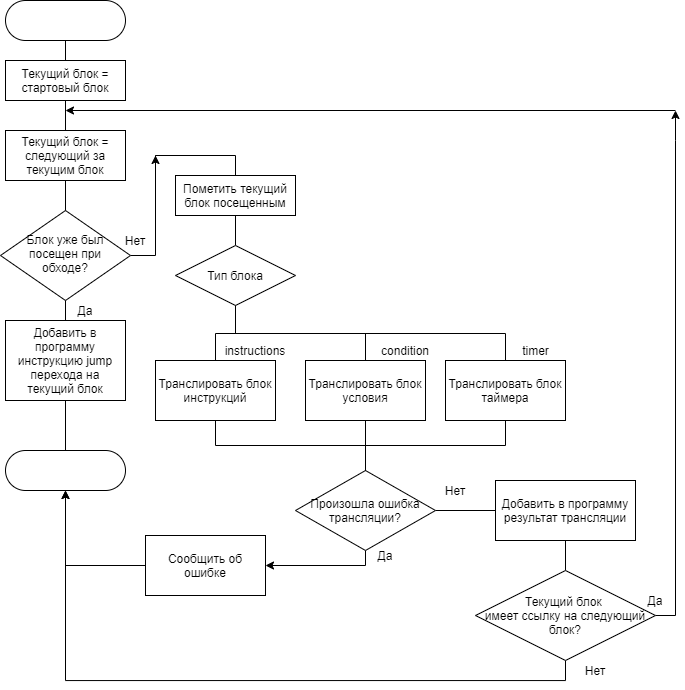
\includegraphics[width=\textwidth]{translator-scheme.png}
	\caption{Схема алгоритма работы транслятора}%
	\label{fig:translator-scheme}
\end{figure}

\subsection{Выполнение программы}

В начале этапа выполнения программы происходит инициализация пользовательских переменных. Для каждой переменной \lstinline|v| выполняется \lstinline|window[v] = 0|. Переменная явно инициализируется типом Number для экономии ресурсов, поскольку формальный синтаксис использует оператор «==» в качестве оператора равенства, который для сравнения приводит типы операндов к общему, в случае, если они не совпадают \cite{mdn-sameness}.

Затем, инициализируется счетчик команд \lstinline|this.PC = 0| и запускается цикл выполнения. В этом цикле каждая инструкция помещается в очередь задач с помощью  функции \lstinline|setInterval| с параметром задержки, равном нулю. Такая реализация позволяет параллельно работать модулям выполнения программы и отрисовки модели, не блокируя при этом выполнение сценариев на остальной странице.

Реализация таймера представляет собой отмену цикла выполнения через \lstinline|clearInterval|, с последующим его возобновлением с помощью \lstinline|setTimeout| с параметром задержки, равному содержимому блока «timer».

Цикл выполнения считается завершенным при выходе счетчика команд за границы массива, что, однако не означает окончание процесса симуляции. Так, например, если выполнение программы завершилось, но переменная состояние робота имеет значение, отличное от нуля, робот продолжит движение в заданном направлении, пока не придет либо в область финиша (успешное окончание симуляции), либо не пересечется со стенкой (неуспешное окончание симуляции).

 


%%%%%%%%%%%%%%%%%%%%%%%%%%%%%%%%%%%%%%%%%%%%%%%%%%%%%%%%%%%%%%%%%%%%%%%%%%%%%%%%

%You can review what you have to do in figure~\ref{fig:how-to-do-research}.
%Please do so now.
